\documentclass[review]{elsarticle}

\usepackage{multirow}
\usepackage{lineno}
\usepackage{xspace}
\usepackage{threeparttable}
\usepackage{subfig}
\modulolinenumbers[5]

%% Journal name here
\journal{Journal Title}

%% `Elsevier LaTeX' style
\bibliographystyle{elsarticle-num}
%%%%%%%%%%%%%%%%%%%%%%%

%%%% packages and definitions (optional)
\usepackage{placeins}
\usepackage{booktabs} % nice rules (thick lines) for tables
\usepackage{microtype} % improves typography for PDF
\usepackage{hhline}
\usepackage{amsmath}
\usepackage{subfig}

\usepackage{booktabs}
\usepackage{threeparttable, tablefootnote}

\usepackage{tabularx}
\usepackage{siunitx}

%% Special typesetting for Cyclus
\newcommand{\Cyclus}{\textsc{Cyclus}\xspace}%
\newcommand{\Cycamore}{\textsc{Cycamore}\xspace}%
\graphicspath{{images/}}

% tikz %
\usepackage{tikz}
\usetikzlibrary{positioning, arrows, decorations, shapes}

\usetikzlibrary{shapes.geometric,arrows}
\tikzstyle{process} = [rectangle, rounded corners, minimum width=3cm, minimum height=1cm,text centered, draw=black, fill=blue!30]
\tikzstyle{object} = [ellipse, rounded corners, minimum width=3cm, minimum height=1cm,text centered, draw=black, fill=green!30]
\tikzstyle{arrow} = [thick,->,>=stealth]

% hyperref %
\usepackage[hidelinks]{hyperref}
% after hyperref %
\usepackage{cleveref}
\usepackage{datatool}
\usepackage[acronym,toc]{glossaries}
%\newacronym{<++>}{<++>}{<++>}
\newacronym[longplural={metric tons of heavy metal}]{MTHM}{MTHM}{metric ton of heavy metal}
\newacronym{ABM}{ABM}{agent-based modeling}
\newacronym{ACDIS}{ACDIS}{Program in Arms Control \& Domestic and International Security}
\newacronym{ADS}{ADS}{Accelerator-Driven System}
\newacronym{AFCI}{AFCI}{Advanced Fuel Cycles Initiative}
\newacronym{AHTR}{AHTR}{Advanced High Temperature Reactor}
\newacronym{ANDRA}{ANDRA}{Agence Nationale pour la gestion des D\'echets RAdioactifs, the French National Agency for Radioactive Waste Management}
\newacronym{ANL}{ANL}{Argonne National Laboratory}
\newacronym{ANS}{ANS}{American Nuclear Society}
\newacronym{API}{API}{application programming interface}
\newacronym{ARE}{ARE}{Aircraft Reactor Experiment}
\newacronym{ARFC}{ARFC}{Advanced Reactors and Fuel Cycles}
\newacronym{ASME}{ASME}{American Society of Mechanical Engineers}
\newacronym{ASTRID}{ASTRID}{Advanced Sodium Technological Reactor for Industrial Demonstration}
\newacronym{ATWS}{ATWS}{Anticipated Transient Without Scram}
\newacronym{BDBE}{BDBE}{Beyond Design Basis Event}
\newacronym{BIDS}{BIDS}{Berkeley Institute for Data Science}
\newacronym{BWR}{BWR}{Boiling Water Reactor}
\newacronym{CAFCA}{CAFCA}{ Code for Advanced Fuel Cycles Assessment }
\newacronym{CDTN}{CDTN}{Centro de Desenvolvimento da Tecnologia Nuclear}
\newacronym{CEA}{CEA}{Commissariat \`a l'\'Energie Atomique et aux \'Energies Alternatives}
\newacronym{CI}{CI}{continuous integration}
\newacronym{CNEN}{CNEN}{Comiss\~{a}o Nacional de Energia Nuclear}
\newacronym{CNERG}{CNERG}{Computational Nuclear Engineering Research Group}
\newacronym{COSI}{COSI}{Commelini-Sicard}
\newacronym{COTS}{COTS}{commercial, off-the-shelf}
\newacronym{CSNF}{CSNF}{commercial spent nuclear fuel}
\newacronym{CTAH}{CTAHs}{Coiled Tube Air Heaters}
\newacronym{CUBIT}{CUBIT}{CUBIT Geometry and Mesh Generation Toolkit}
\newacronym{CURIE}{CURIE}{Centralized Used Fuel Resource for Information Exchange}
\newacronym{DAG}{DAG}{directed acyclic graph}
\newacronym{DANESS}{DANESS}{Dynamic Analysis of Nuclear Energy System Strategies}
\newacronym{DBE}{DBE}{Design Basis Event}
\newacronym{DESAE}{DESAE}{Dynamic Analysis of Nuclear Energy Systems Strategies}
\newacronym{DHS}{DHS}{Department of Homeland Security}
\newacronym{DOE}{DOE}{Department of Energy}
\newacronym{DNP}{DNP}{delayed neutron precursors}
\newacronym{DRACS}{DRACS}{Direct Reactor Auxiliary Cooling System}
\newacronym{DRE}{DRE}{dynamic resource exchange}
\newacronym{DSNF}{DSNF}{DOE spent nuclear fuel}
\newacronym{DYMOND}{DYMOND}{Dynamic Model of Nuclear Development }
\newacronym{EBS}{EBS}{Engineered Barrier System}
\newacronym{EDF}{EDF}{Électricité de France}
\newacronym{EDZ}{EDZ}{Excavation Disturbed Zone}
\newacronym{EIA}{EIA}{U.S. Energy Information Administration}
\newacronym{EPA}{EPA}{Environmental Protection Agency}
\newacronym{EPR}{EPR}{European Pressurized Reactor}
\newacronym{EP}{EP}{Engineering Physics}
\newacronym{EU}{EU}{European Union}
\newacronym{EVOL}{EVOL}{Evaluation and Viability of Liquid Fuel Fast Reactor Systems}
\newacronym{FCO}{FCO}{Fuel Cycle Options}
\newacronym{FCT}{FCT}{Fuel Cycle Technology}
\newacronym{FEHM}{FEHM}{Finite Element Heat and Mass Transfer}
\newacronym{FEPs}{FEPs}{Features, Events, and Processes}
\newacronym{FHR}{FHR}{Fluoride-Salt-Cooled High-Temperature Reactor}
\newacronym{FLiBe}{FLiBe}{Fluoride-Lithium-Beryllium}
\newacronym{FP}{FP}{Fission Products}
\newacronym{GDSE}{GDSE}{Generic Disposal System Environment}
\newacronym{GDSM}{GDSM}{Generic Disposal System Model}
\newacronym{GENIUSv1}{GENIUSv1}{Global Evaluation of Nuclear Infrastructure Utilization Scenarios, Version 1}
\newacronym{GENIUSv2}{GENIUSv2}{Global Evaluation of Nuclear Infrastructure Utilization Scenarios, Version 2}
\newacronym{GENIUS}{GENIUS}{Global Evaluation of Nuclear Infrastructure Utilization Scenarios}
\newacronym{GIF}{GIF}{Generation IV International Forum}
\newacronym{GPAM}{GPAM}{Generic Performance Assessment Model}
\newacronym{GRSAC}{GRSAC}{Graphite Reactor Severe Accident Code}
\newacronym{GUI}{GUI}{graphical user interface}
\newacronym{HLW}{HLW}{high level waste}
\newacronym{HPC}{HPC}{high-performance computing}
\newacronym{HTC}{HTC}{high-throughput computing}
\newacronym{HTGR}{HTGR}{High Temperature Gas-Cooled Reactor}
\newacronym{IAEA}{IAEA}{International Atomic Energy Agency}
\newacronym{IEMA}{IEMA}{Illinois Emergency Mangament Agency}
\newacronym{IHLRWM}{IHLRWM}{International High Level Radioactive Waste Management}
\newacronym{INL}{INL}{Idaho National Laboratory}
\newacronym{IPRR1}{IRP-R1}{Instituto de Pesquisas Radioativas Reator 1}
\newacronym{IRP}{IRP}{Integrated Research Project}
\newacronym{ISFSI}{ISFSI}{Independent Spent Fuel Storage Installation}
\newacronym{ISRG}{ISRG}{Independent Student Research Group}
\newacronym{JFNK}{JFNK}{Jacobian-Free Newton Krylov}
\newacronym{LANL}{LANL}{Los Alamos National Laboratory}
\newacronym{LBNL}{LBNL}{Lawrence Berkeley National Laboratory}
\newacronym{LCOE}{LCOE}{levelized cost of electricity}
\newacronym{LDRD}{LDRD}{laboratory directed research and development}
\newacronym{LFR}{LFR}{Lead-Cooled Fast Reactor}
\newacronym{LLNL}{LLNL}{Lawrence Livermore National Laboratory}
\newacronym{LMFBR}{LMFBR}{Liquid Metal Fast Breeder Reactor}
\newacronym{LOFC}{LOFC}{Loss of Forced Cooling}
\newacronym{LOHS}{LOHS}{Loss of Heat Sink}
\newacronym{LOLA}{LOLA}{Loss of Large Area}
\newacronym{LP}{LP}{linear program}
\newacronym{LWR}{LWR}{Light Water Reactor}
\newacronym{MAGNOX}{MAGNOX}{Magnesium Alloy Graphie Moderated Gas Cooled Uranium Oxide Reactor}
\newacronym{MA}{MA}{minor actinide}
\newacronym{MCNP}{MCNP}{Monte Carlo N-Particle code}
\newacronym{MILP}{MILP}{mixed-integer linear program}
\newacronym{MIT}{MIT}{the Massachusetts Institute of Technology}
\newacronym{MOAB}{MOAB}{Mesh-Oriented datABase}
\newacronym{MOOSE}{MOOSE}{Multiphysics Object-Oriented Simulation Environment}
\newacronym{MOX}{MOX}{Mixed Oxide Fuel}
\newacronym{MPM}{MPM}{Multi-Physics Modelling}
\newacronym{MSBR}{MSBR}{Molten Salt Breeder Reactor}
\newacronym{MSFR}{MSFR}{Molten Salt Fast Reactor}
\newacronym{MSRE}{MSRE}{Molten Salt Reactor Experiment}
\newacronym{MSR}{MSR}{Molten Salt Reactor}
\newacronym{MWe}{MWe}{Megawatts electric}
\newacronym{NAGRA}{NAGRA}{National Cooperative for the Disposal of Radioactive Waste}
\newacronym{NEAMS}{NEAMS}{Nuclear Engineering Advanced Modeling and Simulation}
\newacronym{NEUP}{NEUP}{Nuclear Energy University Programs}
\newacronym{NFCSim}{NFCSim}{Nuclear Fuel Cycle Simulator}
\newacronym{NGNP}{NGNP}{Next Generation Nuclear Plant}
\newacronym{NMWPC}{NMWPC}{Nuclear MW Per Capita}
\newacronym{NNSA}{NNSA}{National Nuclear Security Administration}
\newacronym{NPRE}{NPRE}{Department of Nuclear, Plasma, and Radiological Engineering}
\newacronym{NQA1}{NQA-1}{Nuclear Quality Assurance - 1}
\newacronym{NRC}{NRC}{Nuclear Regulatory Commission}
\newacronym{NSF}{NSF}{National Science Foundation}
\newacronym{NSSC}{NSSC}{Nuclear Science and Security Consortium}
\newacronym{NUWASTE}{NUWASTE}{Nuclear Waste Assessment System for Technical Evaluation}
\newacronym{NWF}{NWF}{Nuclear Waste Fund}
\newacronym{NWTRB}{NWTRB}{Nuclear Waste Technical Review Board}
\newacronym{OCRWM}{OCRWM}{Office of Civilian Radioactive Waste Management}
\newacronym{ORION}{ORION}{ORION}
\newacronym{ORNL}{ORNL}{Oak Ridge National Laboratory}
\newacronym{PARCS}{PARCS}{Purdue Advanced Reactor Core Simulator}
\newacronym{PBAHTR}{PB-AHTR}{Pebble Bed Advanced High Temperature Reactor}
\newacronym{PBFHR}{PB-FHR}{Pebble-Bed Fluoride-Salt-Cooled High-Temperature Reactor}
\newacronym{PDE}{PDE}{partial differential equation}
\newacronym{PEI}{PEI}{Peak Environmental Impact}
\newacronym{PHWR}{PHWR}{Pressurized Heavy Water Reactor}
\newacronym{PH}{PRONGHORN}{PRONGHORN}
\newacronym{PRIS}{PRIS}{Power Reactor Information System}
\newacronym{PRKE}{PRKE}{Point Reactor Kinetics Equations}
\newacronym{PSPG}{PSPG}{Pressure-Stabilizing/Petrov-Galerkin}
\newacronym{PWAR}{PWAR}{Pratt and Whitney Aircraft Reactor}
\newacronym{PWR}{PWR}{Pressurized Water Reactor}
\newacronym{PyNE}{PyNE}{Python toolkit for Nuclear Engineering}
\newacronym{PyRK}{PyRK}{Python for Reactor Kinetics}
\newacronym{QA}{QA}{quality assurance}
\newacronym{RANS}{RANS}{Reynolds-averaged Navier-Stokes}
\newacronym{RDD}{RD\&D}{Research Development and Demonstration}
\newacronym{RD}{R\&D}{Research and Development}
\newacronym{RELAP}{RELAP}{Reactor Excursion and Leak Analysis Program}
\newacronym{RIA}{RIA}{Reactivity Insertion Accident}
\newacronym{RIF}{RIF}{Region-Institution-Facility}
\newacronym{SAMOFAR}{SAMOFAR}{Safety Assessment of the Molten Salt Fast Reactor}
\newacronym{SFR}{SFR}{Sodium-Cooled Fast Reactor}
\newacronym{SINDAG}{SINDA{\textbackslash}G}{Systems Improved Numerical Differencing Analyzer $\backslash$ Gaski}
\newacronym{SKB}{SKB}{Svensk K\"{a}rnbr\"{a}nslehantering AB}
\newacronym{SNF}{SNF}{spent nuclear fuel}
\newacronym{SNL}{SNL}{Sandia National Laboratory}
\newacronym{STC}{STC}{specific temperature change}
\newacronym{SUPG}{SUPG}{Streamline-Upwind/Petrov-Galerkin}
\newacronym{SWF}{SWF}{Separations and Waste Forms}
\newacronym{SWU}{SWU}{Separative Work Unit}
\newacronym{TRIGA}{TRIGA}{Training Research Isotope General Atomic}
\newacronym{TRISO}{TRISO}{Tristructural Isotropic}
\newacronym{TSM}{TSM}{Total System Model}
\newacronym{TSPA}{TSPA}{Total System Performance Assessment for the Yucca Mountain License Application}
\newacronym{ThOX}{ThOX}{thorium oxide}
\newacronym{UFD}{UFD}{Used Fuel Disposition}
\newacronym{UML}{UML}{Unified Modeling Language}
\newacronym{UNF}{UNF}{Used Nuclear Fuel}
\newacronym{UOX}{UOX}{Uranium Oxide Fuel}
\newacronym{UQ}{UQ}{uncertainty quantification}
\newacronym{US}{US}{United States}
\newacronym{UW}{UW}{University of Wisconsin}
\newacronym{VISION}{VISION}{the Verifiable Fuel Cycle Simulation Model}
\newacronym{VVER}{VVER}{Voda-Vodyanoi Energetichesky Reaktor (Russian Pressurized Water Reactor)}
\newacronym{VV}{V\&V}{verification and validation}
\newacronym{WIPP}{WIPP}{Waste Isolation Pilot Plant}
\newacronym{YMR}{YMR}{Yucca Mountain Repository Site}


\makeglossaries

\begin{document}
\begin{frontmatter}
\title{Coupled Neutronics/Thermal-Hydraulics Analysis of the Molten Salt
Fast Reactor}

%\date{}                     % uncomment if you don't need date to appear

% Authors
\author[uiuc]{Sun Myung Park}
\author[uiuc]{Kathryn D. Huff\corref{corrauthor}}
%% If unsure, google "corresponding author" for more info
\cortext[corrauthor]{Corresponding Author}
\ead{kdhuff@illinois.edu}


% Institutes of the authors
\address[uiuc]{Dept. of Nuclear, Plasma, and Radiological Engineering, University of Illinois at Urbana-Champaign, Urbana, IL 61801}


\begin{keyword}
molten salt reactor \sep
molten salt fast reactor \sep
multiphysics \sep
safety analysis \sep 
reactor dynamics \sep
high performance computing
\end{keyword}

\begin{abstract}
The abstract goes here. As a general guide, you should provide a concise
(150-250 words) summary of your article - introduction, methodology, results,
and conclusion. Avoid using abbreviations and acronyms unless the
abbreviation/acronym is used repeatedly in the abstract. There should be no
references in the abstract.
\end{abstract}

\end{frontmatter}
\glsresetall

%% Shows line numbers
\linenumbers

\section{Introduction}

The \gls{MSR} concept is one of the six advanced nuclear reactor concepts
shortlisted by the \gls{GIF} for improved safety, sustainability, efficiency
and cost over the current generations of reactors
\cite{gif_technology_2002} \cite{gif_technology_2014}. This has led
to growing
research interest in \glspl{MSR} in the past two decades, after a relative
lull that followed shortly after the shutdown of the first and only fully
operational \gls{MSR} reactors, the \gls{ARE} and \gls{MSRE}, back in the
1950s and 1960s \cite{haubenreich_msre_1964}
\cite{haubenreich_experience_1970}. In particular, \glspl{MSR} concepts boast
significant advantages in reactor safety and sustainability arising from the
liquid fuel form \cite{elsheikh_safety_2013}. The thermal expansion of the
fuel contributes significantly to the
strongly negative temperature reactivity coefficients observed in most
\gls{MSR} designs. In the event of a power excursion and the accompanying
temperature rise, this reactivity feedback is quite prompt and limits the
maximum temperature that the reactor may reach during this type of accident
scenario. Using liquid fuel also allows for continuous online reprocessing
which impacts sustainability in two main ways: increasing overall fuel burnup
through the continuous removal of parasitic fission products and minimal
downtime, and improving breeding ratios in the context of the thorium fuel
cycle where the intermediate Pa is temporarily removed from the reactor core
to prevent the undesirable formation of U234.

However, this new feature also brought about novel computational
challenges in simulating the transient behavior of \glspl{MSR}; the
neutronics and thermal-hydraulics are more tightly coupled due to the strong
temperature reactivity coefficient, and the additional advection coupling
terms. Furthermore, we have to account for the movement of \glspl{DNP} as
they are now generated directly within the primary coolant loop. Therefore,
the choice of coupling methods for each set of physics requires careful
consideration. Existing reactor system-level codes and modeling approaches
for conventional \glspl{LWR} analysis contain simplifying assumptions in
multiphysics coupling and other areas that render the techniques unsuitable
for simulating \gls{MSR}. Thus, making minor modifications to these codes
without changing the underlying algorithms is not the best approach for
\gls{MSR} safety analysis.

In the past two decades, researchers have developed several
new tools for simulating steady-state and transient behavior in \glspl{MSR}.
Many of the earlier efforts featured simplifications in simulating
thermal-hydraulics by solving 1-D Navier-Stokes equations or using
predetermined uniform velocity fields \cite{krepel_dyn3d-msr_2007}
\cite{kophazi_development_2009}. In more recent years, there has been
significant progress towards fully coupled, spatial codes that feature
2-D axisymmetric or full 3-D models. In 2011, Cammi et al.
\cite{cammi_multi-physics_2011} performed an ``\gls{MPM}'' analysis
of a simplified 2-D axisymmetric model of a single MSBR fuel channel using
the commercial finite-element analysis software COMSOL Multiphysics. The
physics were implemented through the two-group neutron diffusion
equations, and the \gls{RANS} standard $k-\epsilon$ turbulence model, for the
neutronics and thermal-hydraulics respectively. The
authors emphasized the need for proper full coupling of the multiphysics, and
presented both steady-state and transient results in various
scenarios such as reactivity insertions, changes in pumping rate, and the
presence of periodic perturbations. This approach featured again in a later
paper by Fiorina et al. \cite{fiorina_modelling_2014} in 2014 for a 2-D
axisymmetric model of the
\gls{MSFR}. The authors presented results from the Politecnico di Milano
COMSOL-based approach, and another approach by researchers from Delft
University of Technology, where they coupled their in-house neutronics and
thermal-hydraulics codes, DALTON and HEAT respectively. With multi-group
neutron diffusion and \gls{RANS} formulations on ultra-fine meshes, both
models showed good agreement in the steady-state neutron flux, temperature,
and \gls{DNP} distributions, and in the power responses following various
accident transient initiations. Aufiero et al. \cite{aufiero_development_2014}
concurrently developed
a full-core 3-D model of the \gls{MSFR} on OpenFOAM, albeit with one-group
neutron diffusion to reduce computational load. With the 3-D model, the
authors could simulate the asymmetric reactor response to the failure of a
single pump in the sixteen-pump \gls{MSFR} configuration. The authors also
provided some quantitative data supporting the use of implicit coupling over
explicit coupling to obtain accurate solutions of the transient cases.
Recognizing the huge computational burden required for full 3-D simulations, 
later authors came up with innovative ways to alleviate this issue such as
selective geometrical reduced order modeling for various components of a
reactor based on the importance of the physical phenomena being simulated
\cite{zanetti_geometric_2015}, or using a novel, efficient method for
neutronics calculations \cite{laureau_transient_2017}.

In this paper, we present steady-state and transient analysis of the
\gls{MSFR} concept using Moltres \cite{lindsay_introduction_2018}, a
multiphysics finite element analysis tool
for simulating \glspl{MSR}. Similar to the COMSOL and OpenFOAM, Moltres
solves the deterministic multi-group neutron diffusion and thermal-hydraulics
\glspl{PDE} simultaneously on the same mesh. It supports up to 3-D meshes and
scales well for an arbitrary number of processors. As a code under active
development, the main objective of this paper is to benchmark Moltres' current
capabilities against similar codes in the context of the reference
\gls{MSFR} concept. A previous study \cite{lindsay_introduction_2018}
showcasing Moltres' capabilities with
the \gls{MSRE} design had shown good agreement with legacy
\gls{MSRE} data and strong parallel performance with up to 768 processors.
We leverage on this powerful feature to provide high fidelity \gls{MSFR}
simulation results at reasonable wall-clock times.

The paper is organized as follows. (Insert paper format)

\section{Molten Salt Fast Reactor}

The \gls{MSFR} is a reference design of a circulating-fuel \gls{MSR} developed
under the EURATOM \gls{EVOL} \cite{euratom_final_2015} and \gls{SAMOFAR}
\cite{kloosterman_20_2017} projects. The core of the
\gls{MSFR} consists of a 9 m$^3$ pool of fuel salt flowing upwards
\cite{serp_molten_2014}. At the top
of the core, the fuel salt flow separates into sixteen individual peripheral
loops, passing through the pumps, heat exchangers, and other instrumentation,
before flowing back into the active core region from the bottom. The core is
surrounded axially by nickel alloy reflectors, and radially by a toroidal
blanket tank containing fertile salt for
breeding. A layer of boron carbide absorber further protects the outer
components from excessive neutron damage. The main reactor specifications and
schematic view are shown in Table \ref{table:msfr} and Fig. \ref{fig:msfr}
respectively. 
%
\begin{table}[htb!]
	\caption{Main specifications of the \gls{MSFR} concept
				\cite{serp_molten_2014}.}
	\centering
	\begin{tabular}{ l r }
		\hline
		Parameter & Value \\
		\hline
		Thermal/Electric output [MW$_{\text{th}}$/MW$_{\text{e}}$] & 3000 /
		1500 
		\\
		Salt volume [m$^3$] & 18 \\
		Salt fraction in core & 0.5 \\
		Number of circulation loops & 16 \\
		Nominal flow rate [kg s$^{-1}$] & 18500  \\
		Nominal circulation time [s] & 4.0 \\
		Inlet/outlet temperature [K] & 923 / 1023 \\
		Blanket volume [m$^3$] & 7.3\\
		\hline
	\end{tabular}
	\label{table:msfr}
\end{table}
%
\begin{figure}[htb!] 
	\centering
	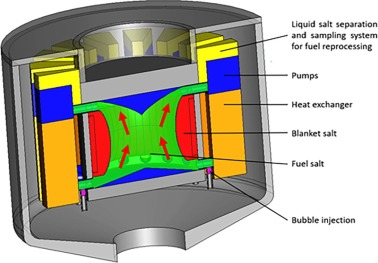
\includegraphics[width=0.6\textwidth]{MSFR}
	\caption{Schematic view of the MSFR concept \cite{serp_molten_2014}.}
	\label{fig:msfr}
\end{figure}

For the $^{232}$Th/$^{233}$U breeder configuration, the fuel and blanket salts
are composed of eutectic mixtures of 77.5\% LiF - 22.5\% AcF$_4$, where
AcF$_4$ represents actinide fluorides, uranium and thorium fluoride
\cite{serp_molten_2014}. A mole
fraction of approximately 1\% $^{233}$U is required for criticality; most
studies adjust the composition to achieve criticality at a uniform temperature
973 K as was done in the \gls{MSFR} neutronics benchmark paper
\cite{brovchenko_neutronic_2019}. Breeding ratios of up to 1.1 are expected
for the \gls{MSFR} \cite{fiorina_molten_2013}.

According to the design specifications, the inlet and outlet temperatures of
the fuel salt are to be 923 K and 1023 K respectively. This was motivated by
the desire for a 50 K minimum buffer between the operating temperatures
and the melting point of the salt \cite{euratom_final_2015}.
Having a secondary coolant loop adds a layer of containment between the
radioactive material and the outside environment. The exact specifications of
the heat exchanger and the secondary coolant loop are yet to be determined.
Thus, we assumed a secondary coolant temperature of 823 K with a heat transfer
coefficient value that corresponds to the intended 100 K temperature drop in
the fuel salt.

\section{Methodology}

This section discusses the geometry and the modeling approach in this paper.
The reactor model geometry in this paper is kept unchanged from the models
used by Fiorina et al. \cite{fiorina_modelling_2014} and Aufiero et al.
\cite{aufiero_development_2014}, henceforth referred to as the
Polimi/TUDelft models, to provide a fair comparison in this
benchmarking exercise.

\subsection{Reactor Model Geometry and Group Constant Generation}

For this work, we used the reference square-cylindrical \gls{MSFR} design to
benchmark Moltres against results published by Fiorina et al. and Aufiero et
al. It is a 2-D axisymmetric design with the sixteen individual external loops
homogenized into a single outer loop as shown in Fig. \ref{fig:msfrgeom}. For
the multi-group
cross sections and group constants calculations in Serpent, we extended this
2-D axisymmetric model into a 3-D model by a simple full rotation about the
central axis. The material definitions are the same as those specified in the
reference \gls{MSFR} model. Accordingly, the pump and heat exchanger regions
are assumed to be composed of 100\% fuel salt. While this may not be entirely
accurate, the exact details of the pump and heat exchanger systems are still
be researched, and this external loop region is presumed to be of little
neutronic importance due to its position behind the strong boron carbide
neutron absorber layer.
%
\begin{figure}[htb!] 
	\centering
	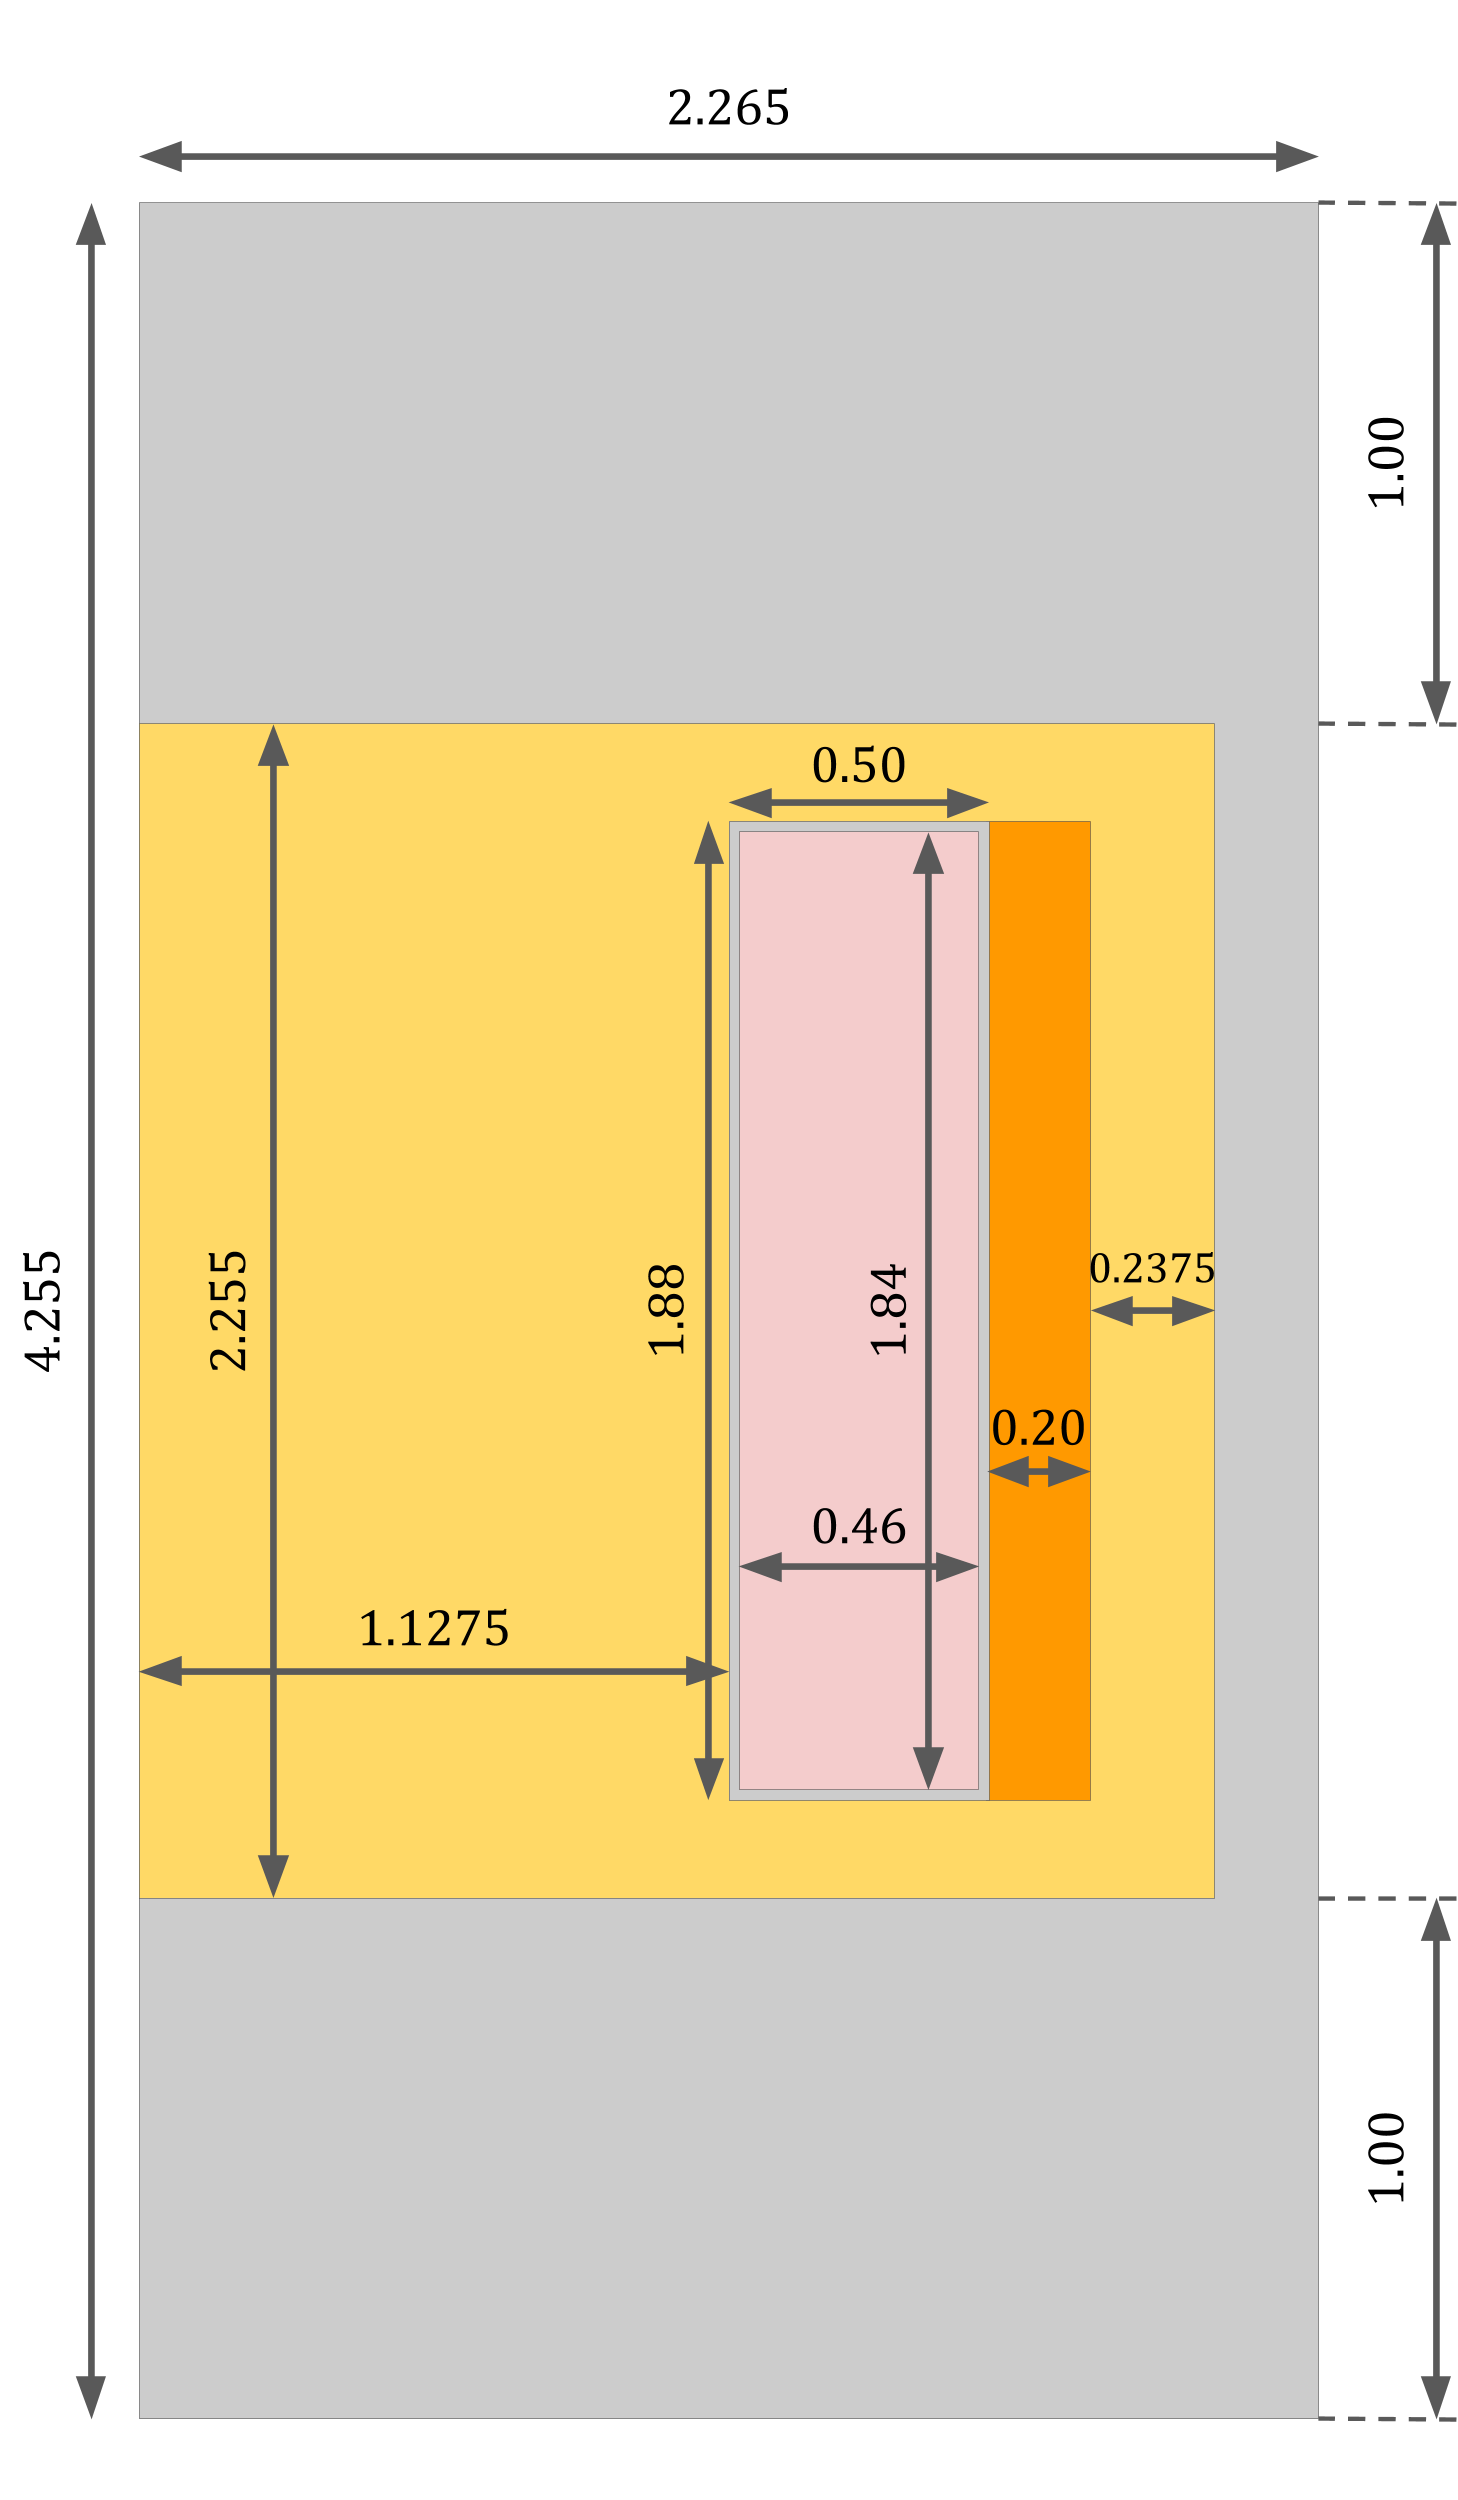
\includegraphics[width=0.5\textwidth]{msfr-geom}
	\caption{2-D axisymmetric model of the \gls{MSFR} core used for the
	simulations in Serpent and Moltres. All dimensions are in meters.
	\cite{brovchenko_neutronic_2019}}
	\label{fig:msfrgeom}
\end{figure}

There are two key differences between our \gls{MSFR} model geometry in
Moltres and the Polimi/TUDelft models. The first difference is a relative
minor change to the mesh by the exclusion of the 2 cm thick structural
material around the blanket tank that separates the fuel and blanket salts.
We removed this feature in our finite element mesh as we had difficulty
meshing this layer that is relatively much thinner than the rest of the model.
Any impact on the
neutron flux is expected to be minimal. Furthermore, we solved for the
temperature distribution only in the primary loop and applied homogeneous
Neumann boundary conditions for temperature on the core walls, as was done in
the Polimi/TUDelft models. Therefore, we believe the overall impact on the
results is negligible.

The second difference pertains to the modeling of the external loop. In its
current implementation, Moltres lacks pump- and heat exchanger-equivalents in
the code. Thus, the external loop is modeled as a 1-D pipe with a point heat
sink to represent the heat exchanger. Instead of pumps, the flow is driven by
Dirichlet boundary conditions for velocity on the inlet and outlet boundaries
of the 2-D axisymmetric central core geometry and the 1-D external pipe
geometry. All flow-dependent variables such as temperature, \glspl{DNP}, and
decay heat precursors are fully conserved as they loop around between the two
regions. As a result, this approach shares some similarities with the
geometric multiscale modeling approach by Zanetti et al.
\cite{zanetti_geometric_2015} Future models could
create a better representation of the primary loop by implementing a whole
continuous loop with pressure increases and drops corresponding to the pumps
and heat exchangers. 

We used the JEFF-3.1.2 cross-section library \cite{oecd/nea_jeff-3.1.2_2014}
for group constant generation in
Serpent. We set a neutron population of 200,000 neutrons per cycle with 50
inactive and 500 active cycles for a total of 100 million neutron histories.
The material compositions of the various reactor components follows the
benchmark specification, with slight adjustments to the
ratio of $^{232}$Th to $^{233}$U to obtain $k_{\text{eff}}=1$ at 973 K. The
resulting mole fraction is very close to a result cited in the neutronics
benchmark paper which was also generated from Serpent using the JEFF-3.1.1
library (Table \ref{table:mole}). The differences can be largely attributed to
the statistical uncertainty for both results. We divided the primary loop into
3 subdivisions: core, inlet/outlet, and heat pump/exchanger regions. This was
motivated by the difference in neutronic importance of those regions. We
followed the same six-group
structure (Table \ref{table:bound}) as the Polimi COMSOL model
\cite{fiorina_modelling_2014}. The
energy boundaries for the six neutron energy groups are shown in Table
\ref{table:bound}. For the \glspl{DNP}, the JEFF-3.1.2 library provides
eight pre-defined \gls{DNP} groups based on their half-lives. The relevant
group constants for Moltres simulations are: the various macroscopic neutron
cross-sections, neutron diffusion coefficient, average fission energy, average
neutron yield, inverse neutron speed, fission spectrum, \gls{DNP} group
constants, and effective delayed neutron fractions.

Moltres, by extension from MOOSE, accepts various mesh file formats; we refer
readers to the MOOSE framework website for the full list of supported file
formats. We used the Trelis 16.5 \cite{noauthor_trelis_2018} to generate the
\gls{MSFR} mesh (Fig. \ref{fig:msfrgeom}) in this work. There are finer mesh
elements around the absorber region boundaries to accurately capture the steep
drop in neutron flux at those boundaries.
%
\begin{table}[htb!]
	\centering
    \caption{Comparison of mole fractions and $k_{\text{eff}}$ uncertainty
    of $^{232}$Th and $^{233}$U in
    the fuel salt composition adjusted for $k_{eff}=1$ at 973 K.}
\begin{tabular}{l S S}
	\hline
	\textbf{Property} & \textbf{This paper} & \textbf{Benchmark
	\cite{brovchenko_neutronic_2019}} \\
	\hline
    $^{232}$Th mol\% & 19.943 \% & 19.948 \% \\
    $^{233}$U mol\% & 2.557 \% & 2.551 \% \\
    $k_{\text{eff}}$ uncertainty & 4.9 pcm & 4.6 pcm \\
    \hline
\end{tabular}
\label{table:mole}
\end{table}
%
\begin{table}[htb!]
	\centering
	\caption{Neutron energy group upper bounds used in Serpent.}
	\begin{tabular}{c S}
		\hline
		{Group number} & {Upper bound [MeV]}\\
		\hline
		1 & 7.485$\times 10^{-4}$\\
		2 & 5.5308$\times 10^{-3}$\\
		3 & 2.47875$\times 10^{-2}$\\
		4 & 0.4979\\
		5 & 2.2313\\
		6 & 12\\
		\hline
	\end{tabular}
	\label{table:bound}
\end{table}
%
\subsection{Modeling Approach}

Moltres is an application built on the MOOSE \cite{gaston_physics-based_2015}
framework. MOOSE provides a simplified interface for developing fully
coupled multiphysics solvers while leveraging on sophisticated computational
tools: PETSc \cite{satish_petsc_2019}, a non-linear solver package, and
libMesh \cite{kirk_libmesh:_2006}, a finite element library. In Moltres, the
various physical phenomena described by each term in the \glspl{PDE} are
represented by ``kernels'' and boundary conditions. For
example, the individual terms for neutron diffusion, removal, scattering, etc.
each have their own representative kernel. Kernels provide weak
form representations in MOOSE through the calculation of residual and Jacobian
contributions of the corresponding physics. Multiple kernels from the same
\gls{PDE} may also be grouped together for ease of implementation. The neutron
flux and velocity variables were approximated by first-order
Lagrangian finite element shape functions, while the \gls{DNP} and decay heat
precusor variables were approximated by constant monomial shape functions.

\subsubsection{Neutronics}

The neutronics is implemented through the deterministic multi-group neutron
diffusion equations. Due to its modular structure, Moltres can solve for an
arbitrary number of neutron and \gls{DNP} group. Moltres requires group
constant data from dedicated neutron transport codes such as Serpent or SCALE
\cite{dehart_reactor_2011}, and there are python scripts available on the
Moltres GitHub repository \cite{lindsay_moltres_2017} to convert the
Serpent/SCALE output file into a Moltres-compatible format.

The governing equation for time-dependent multi-group neutron diffusion in
Moltres is:
%
\begin{align}
	\frac{1}{v_g} &\frac{\partial \phi_g}{\partial t} - \nabla \cdot D_g
	\nabla \phi_g + \Sigma^r_g \phi_g \nonumber \\ 
	&= \sum^G_{g \neq g'} \Sigma^s_{g' \rightarrow g} \phi_{g'} + \chi^p_g
	\sum^G_{g'=1} (1-\beta) \nu \Sigma^f_{g'} \phi_{g'} + \chi^d_g \sum^I_i
	\lambda_i C_i. \label{eq1}
\end{align}
%	\intertext{where}
%	v_g &= \text{average speed of neutrons in group }g \nonumber \\
%	\phi_g &= \text{flux of neutrons in group }g \nonumber \\
%	t &= \text{time} \nonumber \\
%	D_g &= \text{diffusion coefficient of neutrons in group }g \nonumber \\
%	\Sigma^R_g &= \text{macroscopic cross-section for removal of neutrons} 
%	\nonumber \\
%	&\text{from group }g \nonumber \\
%	\Sigma^s_{g' \rightarrow g} &= \text{macroscopic cross-section of
%	scattering from }g' \text{ to }g \nonumber \\
%	\chi^p_g &= \text{prompt fission spectrum neutrons in group }g \nonumber
%	\\
%	G &= \text{number of discrete neutron groups, }g \nonumber \\
%	\nu &= \text{average number of neutrons produced per fission} \nonumber \\
%	\Sigma^f_{g} &= \text{macroscopic fission cross-section} \nonumber \\
%	&\text{for neutron in group }g \nonumber \\
%	\chi^d_g &= \text{delayed fission spectrum neutrons in group }g \nonumber
%	\\
%	I &= \text{number of delayed neutron precursor groups} \nonumber \\
%	\beta &= \text{delayed neutron fraction} \nonumber \\
%	\lambda_i &= \text{average decay constant of delayed neutron} \nonumber \\
%	&\text{precursors in precursor group }i \nonumber \\
%	C_i &= \text{concentration of delayed neutron precursors} \nonumber \\
%	&\text{in precursor group }i. \nonumber
%\end{align}

We used six energy groups with the cross sections generated on Serpent for
temperatures from 900 K to 1200 K at 50 K intervals. Moltres contains various
interpolation methods for the cross sections for temperatures that fall
between the given temperatures; we applied the spline method for this work.
The temperature dependence of the cross sections from Serpent encompasses both
the Doppler effect and density dependence. We assumed vacuum boundary
conditions for all six neutron groups along the external boundaries of the
geometry and homogeneous Neumann boundary conditions along the axial boundary.

The \glspl{DNP} are governed by the following equation:
%
\begin{align}
	\frac{\partial C_i}{\partial t} = - \nabla(\overrightarrow{u} C_i)
	+ \nabla \cdot \frac{\mu_T}{\rho Sc_T} \nabla C_i	
	- \lambda_i C_i + \sum^G_{g'=1} \beta_i \nu \Sigma^f_{g'}
	\phi_{g'}. \label{eq2}
\end{align}

There are eight \gls{DNP} groups with decay constants pre-defined by the
JEFF-3.1.2 library \cite{oecd/nea_jeff-3.1.2_2014}. Similar to the
Polimi/TUDelft models, the \gls{DNP} equation (Eq. \ref{eq2}) contains both
convective and diffusive terms. The diffusive term arises from turbulent
diffusion approximated by the turbulent viscosity, and the turbulent Schmidt
number assumed to be 0.85. The turbulent viscosity is discussed in greater
detail in the thermal-hydraulics subsection. The \glspl{DNP} are simulated
only in the central core region and the 1-D pipe representing the external
loop. Homogeneous Neumann boundary conditions were applied along the walls of
the central core region, and inflow and outflow boundary conditions were
applied on the inlet and outlet boundaries respectively. We used a prescribed
velocity value in the 1-D external loop region to simulate the time that the
precusors spend outside of the core.

We also included a decay heat model based on a previous work
\cite{aufiero_extended_2013} on the \gls{MSFR}, which found that using three
decay heat precursor groups could model decay heat in the \gls{MSFR} for up to
300 seconds after a full shutdown with less than 2 \% relative error
\cite{aufiero_development_2014}. The decay heat parameters are shown in Table
\ref{table:decay}.

\begin{table}[htb!]
	\centering
	\caption{Decay heat group parameters \cite{fiorina_modelling_2014}.
	$\lambda_i$ and $f_i$ are the decay constants and decay heat fractions
	associated to group $i$.}
	\begin{tabular}{S S S}
		\hline
		{Decay heat group} & {$\lambda_i$ [s$^{-1}$]} & {$f_i$} \\
		\hline
		1 & 0.1974 & 0.0117 \\
		2 & 0.0168 & 0.0129 \\
		3 & 3.58 $\times 10^{-4}$ & 0.0186 \\
		\hline
	\end{tabular}
	\label{table:decay}
\end{table}

\subsubsection{Thermal-hydraulics}



\begin{figure}[htb!]
        \centering
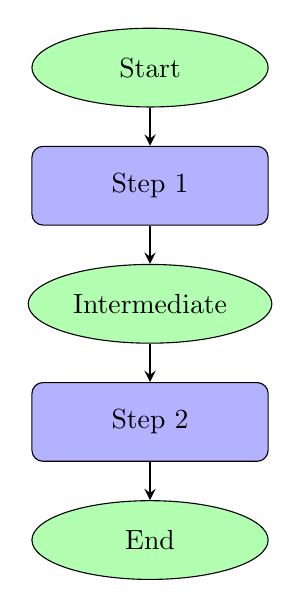
\begin{tikzpicture}[node distance=1.5cm]
\node (start) [object] {Start};
\node (step1) [process, below of=start] {Step 1};
\node (intermediate) [object, below of=step1] {Intermediate};
\node (step2) [process, below of=intermediate] {Step 2};
\node (end) [object, below of=step2]{End};

\draw [arrow] (start) -- (step1); 
\draw [arrow] (step1) -- (intermediate);
\draw [arrow] (intermediate) -- (step2); 
\draw [arrow] (step2) -- (end);
\end{tikzpicture}
\caption{A caption for the flowchart.}
\label{fig:comp}
\end{figure}

\section{Results}

This is the results section.

\begin{align}
	F &= ma \\
	\intertext{where:}
	F &= \text{net force applied on the body [N]} \nonumber \\
	m &= \text{total mass of the body [kg]} \nonumber \\
	a &= \text{net acceleration of the body [m s}^{-2}\text{]} \nonumber
\end{align}

\begin{figure}[htbp!]
	\begin{center}
		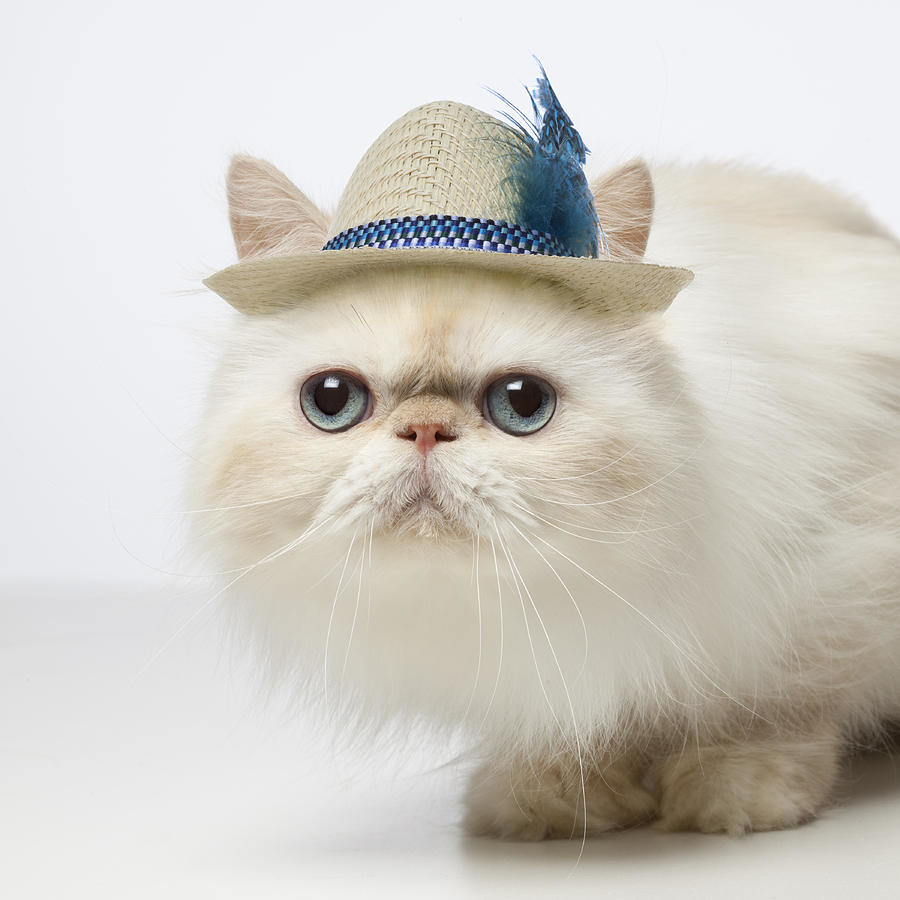
\includegraphics[scale=0.7]{./images/catinhat}
	\end{center}
	\caption{A caption for the figure.}
	\label{fig:catinhat}
\end{figure}

\begin{table}[h]
	\centering
        \caption{A caption for the table.}
\begin{tabular}{lr}
	\hline
	\textbf{Properties} & \textbf{Value} \\
	\hline
    Mass [kg] & 2,324 \\
    Height [m] & 558 \\
    Volume [m$^3$] & 4,072 \\
    \hline
\end{tabular}
\label{tab:table1}
\end {table}

\section{Conclusion}
This is the conclusion section.

Reprocessing schemes also require intensive research because
of the various constraints pertaining to maintaining reactor criticality,
operational safety, and favorable salt redox conditions while maximizing
breeding ratios.

\section{Acknowledgments}
This is the acknowledgements section.
Include acknowledgements for relevant funding sources and contributors for
this work. Review the [how-to-acknowledge] \url{https://drive.google.com/open?id=1VybV0oMPiqpInTwgO0ICq0EC4AL_fGj-zbXGJAhRiVU}
document for the appropriate text, which changes frequently as grants and people
come and go.


\bibliography{bibliography.bib}

% Prof. Huff discourages appendices in journal articles.
% But, if you must, include one like so:
%\pagebreak
%
\appendix
\section{}


\end{document}
